\documentclass[10pt, a4paper]{article}
\usepackage[utf8]{inputenc}
\usepackage[T1]{fontenc}
\usepackage[margin=0.75in]{geometry}
\usepackage[table]{xcolor}
\usepackage{titlesec}
\usepackage{enumitem}
\usepackage{array}
\usepackage{tabularx}
\usepackage{longtable}
\usepackage{booktabs}
\usepackage{hyperref}
\usepackage{graphicx}
\usepackage{float}
\usepackage{tikz}
\usetikzlibrary{positioning}
\usepackage{fancyhdr}
\usepackage{helvet}
\usepackage{setspace}
\renewcommand{\familydefault}{\sfdefault}
\setstretch{1.18}

% Color Definitions -- matched to the source Westcliff University syllabi
\definecolor{primary}{RGB}{1, 38, 89}       % Westcliff Navy (logo / heading text)
\definecolor{secondary}{RGB}{0, 112, 192}   % Westcliff Blue (section bars, links, accents)
\definecolor{midblue}{RGB}{79, 129, 189}    % Mid Blue (rules, borders)
\definecolor{darkgray}{RGB}{50, 50, 50}
\definecolor{lightgray}{RGB}{167, 192, 222} % Westcliff table-row tint
\definecolor{bordergray}{RGB}{210, 215, 225}

% Hyperlink Setup
\hypersetup{
    colorlinks=true,
    linkcolor=primary,
    urlcolor=secondary,
    pdftitle={Combined Syllabus: CLD 400 (Virtualization \& Storage) and TECH 400 (Introduction to Information Retrieval)}
}

% Page Layout & Header
\pagestyle{fancy}
\fancyhf{}
\lhead{\small \textbf{Westcliff University} | Presidential Graduate School}
\rhead{\small \textbf{CLD 400 \& TECH 400} Combined Intensive Syllabus}
\cfoot{\thepage}
\renewcommand{\headrulewidth}{0.4pt}

% Section Formatting: full-width colored bars for top-level sections, matching
% the source syllabi's blue section-header bars.
\newcommand{\sectionbar}[1]{%
  \par\vspace{0.7em}
  \refstepcounter{section}%
  \noindent\colorbox{secondary}{\parbox{\dimexpr\textwidth-2\fboxsep\relax}{\centering\color{white}\bfseries\Large #1}}%
  \par\vspace{0.5em}
}
\titleformat{\subsection}{\large\bfseries\color{primary}}{}{0em}{}
\titleformat{\subsubsection}{\bfseries\color{primary}}{}{0em}{}

% Weekly report callout: #1 = week label, #2 = CLD 400 description, #3 = TECH 400 description
\newcommand{\weeklyreport}[3]{%
  \par\vspace{0.4em}
  \noindent\colorbox{lightgray!35}{\parbox{\dimexpr\textwidth-2\fboxsep\relax}{%
    \textbf{\color{primary}#1 Report} \textit{(separate PDF/DOC per team, theory + lab, per Section~\ref{sec:reporting})}
    \begin{itemize}
        \item \textbf{CLD 400:} #2
        \item \textbf{TECH 400:} #3
    \end{itemize}
  }}%
  \par\vspace{0.3em}
}

\setlist{itemsep=3pt, topsep=4pt, parsep=2pt}

\begin{document}

% ==========================================
% HEADER BLOCK WITH LOGOS
% ==========================================
\begin{center}
    \begin{minipage}[c]{0.22\textwidth}
        \centering
        
\includegraphics[width=2.6cm,keepaspectratio]{images/westcliff_email_logo.png}
    \end{minipage}
    \hfill
    \begin{minipage}[c]{0.52\textwidth}
        \centering
        {\LARGE \textbf{\color{primary} WESTCLIFF UNIVERSITY}}\\[0.2em]
        {\large \textbf{\color{secondary} College of Technology \& Engineering}}\\[0.3em]
        {\small \textit{In Partnership with Presidential Graduate School (Nepal)}}\\[0.5em]
        {\small \textbf{Session:} Spring 2026 \quad|\quad \textbf{Modality:} 6 Hrs/Week \quad|\quad \textbf{Duration:} 8 Weeks}
    \end{minipage}
    \hfill
    \begin{minipage}[c]{0.22\textwidth}
        \centering
        
\includegraphics[width=2.6cm,keepaspectratio]{images/pgs-logo.png}
    \end{minipage}
\end{center}

\vspace{0.8em}
\hrule height 1.5pt
\vspace{1em}

% ==========================================
% COURSE TITLE BLOCK
% ==========================================
\begin{center}
    {\LARGE \textbf{\color{primary} COMBINED SYLLABUS}}\\[0.3em]
    {\Large \textbf{\color{secondary} CLD 400: Virtualization \& Storage}}\\[0.15em]
    {\large \textbf{\color{darkgray} and}}\\[0.15em]
    {\Large \textbf{\color{secondary} TECH 400: Introduction to Information Retrieval}}\\[0.7em]
    {\small \textit{An Advanced, AI-Era, Project-Based Curriculum}}\\[0.4em]
    \textit{Capstone Focus: A Split-Team Build of a Real-Time Distributed Nepali News Crawler, Hybrid Search Engine, \& GIS Spatial News Platform}
\end{center}

\vspace{1em}

% ==========================================
% COURSE OVERVIEW & PEDAGOGICAL PHILOSOPHY
% ==========================================
\sectionbar{Course Overview \& Pedagogical Philosophy}

Generative and agentic AI have permanently raised the floor of what a graduating infrastructure and information-retrieval engineer must be able to design, defend, and ship. A syllabus built around reading an article and answering a discussion prompt no longer prepares a student for a labor market where an AI assistant can already summarize that same article. This combined curriculum therefore replaces introductory, theory-only assignments with a single continuous, production-grade engineering build: every lecture hour is spent moving one shared system forward, and every assignment is a real system component with real failure modes.

This is a combined course, pairing CLD 400 (Virtualization \& Storage) with TECH 400 (Introduction to Information Retrieval) around one shared engineering build, delivered as an 8-week, 6-hour-per-week studio split across two collaborating teams:
\begin{itemize}
    \item \textbf{CLD 400 --- Systems/DevOps:} bare-metal hypervisors, distributed storage, Linux high availability, container orchestration, distributed queues and databases, and full observability.
    \item \textbf{TECH 400 --- Information Retrieval:} distributed crawlers, a Devanagari NLP pipeline, geographic entity resolution, a robust hybrid lexical/neural, cross-lingual search bar (type in Nepali or English), and an interactive province-to-municipality GIS frontend.
\end{itemize}
The two teams move through three phases together, always graded as separate, subject-specific deliverables:

\begin{table}[H]
\centering
\small
\renewcommand{\arraystretch}{1.3}
\begin{tabularx}{\textwidth}{|>{\bfseries}l|c|X|X|}
\hline
\rowcolor{lightgray}
Phase & Weeks & CLD 400 & TECH 400 \\ \hline
Independent Foundations & 1--4 & Stands up the physical infrastructure on its own track. & Covers the full IR theory syllabus and builds algorithm prototypes; no shared infrastructure exists yet. Both teams still hold a weekly sync (Section~\ref{sec:roles}). \\ \hline
Joint Integration \& Deployment & 5--6 & Exposes its infrastructure as a single, explicit interface (Section~\ref{sec:architecture}: the Shared Resource Contract). & Deploys the joint system onto CLD 400's infrastructure against that interface. \\ \hline
Cloud Migration \& Defense & 7--8 & Mentors the AWS migration and defends the on-premise system's resilience. & Migrates and finalizes the search engine on AWS (individual student cloud accounts provided). \\ \hline
\end{tabularx}
\end{table}

Students are expected -- and encouraged -- to use AI coding assistants as part of a modern engineering workflow (see Section~\ref{sec:ai-policy}); the assessment model is therefore weighted toward live defense, architectural reasoning, and working systems rather than static prose, since those are precisely the skills AI cannot yet substitute for a student.

\vspace{0.5em}
\begin{table}[H]
\centering
\small
\renewcommand{\arraystretch}{1.3}
\begin{tabularx}{\textwidth}{|>{\bfseries}l|X|>{\bfseries}l|X|}
\hline
\rowcolor{lightgray}
Course Code & Full Course Name & Credits & Contact Hours \\ \hline
CLD 400 & Virtualization \& Storage & 3 Units & 3 Hours/Week (Integrated) \\ \hline
TECH 400 & Introduction to Information Retrieval & 3 Units & 3 Hours/Week (Integrated) \\ \hline
Combined Format & Combined Intensive Dual-Course Studio & 6 Units & 6 Hours/Week $\times$ 8 Weeks (Lab + Lecture) \\ \hline
\end{tabularx}
\end{table}

% ==========================================
% COURSE IDENTIFICATION
% ==========================================
\sectionbar{Course Identification \& Description}

\begin{table}[H]
\centering
\small
\renewcommand{\arraystretch}{1.25}
\begin{tabularx}{\textwidth}{|>{\bfseries}l|X|}
\hline
\rowcolor{lightgray}
\multicolumn{2}{|c|}{\textbf{CLD 400 --- Virtualization \& Storage}} \\ \hline
Length of Class & 8 Weeks, matching the Westcliff catalog baseline; delivered here at double the weekly contact hours (6 vs.\ 3) to cover the expanded bare-metal infrastructure curriculum below. \\ \hline
Course Description & Provides a production-grade grounding in virtualization and enterprise storage architecture, taught hands-on against physical bare-metal infrastructure (hypervisors, distributed storage, container orchestration) in the shared hardware lab, with a comparative unit on public cloud providers for cost and scaling trade-offs. \\ \hline
Required Text & No single textbook; curated vendor documentation for Proxmox/ESXi, Ceph, Kubernetes, and Terraform/Ansible, plus whitepapers and RFCs, are provided weekly. \\ \hline
Instructional Method & On-Campus intensive studio in the college hardware lab. \\ \hline
\end{tabularx}

\vspace{0.6em}

\begin{tabularx}{\textwidth}{|>{\bfseries}l|X|}
\hline
\rowcolor{lightgray}
\multicolumn{2}{|c|}{\textbf{TECH 400 --- Introduction to Information Retrieval}} \\ \hline
Length of Class & 8 Weeks, matching the Westcliff catalog baseline; delivered here at double the weekly contact hours (6 vs.\ 3), since the catalog outline only covers roughly the first 4 weeks of this expanded build. \\ \hline
Course Description & Covers the theory, implementation, and evaluation of information retrieval systems -- from Boolean and vector-space models through probabilistic ranking to neural, embedding-based retrieval -- culminating in a full-fledged, geographically aware, cross-lingual search engine (map \emph{and} search bar) rather than toy exercises. \\ \hline
Required Text & Manning, C., Raghavan, P., \& Sch\"utze, H. (2009). \textit{Introduction to Information Retrieval} (Online ed.). Cambridge University Press. Freely available at \url{https://nlp.stanford.edu/IR-book/}. \newline \textit{Supplementary:} Hersh, W. (2020). \textit{Information Retrieval: A Biomedical and Health Perspective} (4th ed.). Springer. \newline Goker, A., \& Davies, J. (2009). \textit{Information Retrieval: Searching in the 21st Century} (1st ed.). Wiley. \\ \hline
Instructional Method & On-Campus intensive studio in the college hardware lab. \\ \hline
\end{tabularx}
\end{table}

% ==========================================
% PREREQUISITES
% ==========================================
\sectionbar{Prerequisites \& Incoming Student Expectations}
\begin{itemize}
    \item \textbf{Programming:} Working proficiency in Python (functions, classes, virtual environments, package management).
    \item \textbf{Systems:} Comfort with the Linux command line (file system, permissions, process management, SSH).
    \item \textbf{Networking:} Familiarity with IP addressing, DNS, and HTTP fundamentals.
    \item \textbf{Mathematics:} Basic linear algebra (vectors, dot products) and probability, sufficient to follow TF-IDF, cosine similarity, and Bayesian ranking derivations.
    \item \textbf{Tooling:} A GitHub account is required from Week 1; Git fundamentals are taught in the first lab if needed, not assumed.
    \item \textbf{Lab Access:} Physical attendance in the shared hardware lab (bare-metal servers, enterprise switches, storage nodes, and a GPU-equipped compute node) is required every session; the infrastructure labs run against shared physical state that cannot be replicated remotely.
\end{itemize}

% ==========================================
% RESOURCES & TECH STACK
% ==========================================
\sectionbar{Required Resources \& Modern Technology Stack}
Beyond the required textbook (Section 2), students provision and operate the following production-grade stack throughout the course. No component is used in isolation -- every row below is a piece of the shared capstone system.

\begin{table}[H]
\centering
\small
\renewcommand{\arraystretch}{1.25}
\begin{tabularx}{\textwidth}{|>{\bfseries}l|X|}
\hline
\rowcolor{lightgray}
Layer & Technologies \\ \hline
Bare-Metal Virtualization & Proxmox VE / VMware ESXi, Linux namespaces \& cgroups, Docker, Podman, bare-metal Kubernetes (K3s / MicroK8s) \\ \hline
GPU Compute (CLD 400 only) & NVIDIA GPU node, CUDA/cuDNN, PCI passthrough (VFIO) / vGPU / MIG, Kubernetes NVIDIA device plugin \\ \hline
Networking \& High Availability & VLAN segmentation, LACP NIC bonding, Keepalived + Virtual IPs, HAProxy, Nginx/Traefik ingress, MetalLB \\ \hline
Distributed Storage & Ceph (S3-compatible object gateway) or TrueNAS/NFS, RAID 10/6, PostgreSQL + PostGIS (master-replica) \\ \hline
Queueing \& Search Infrastructure & Redis Cluster / Apache Kafka, Elasticsearch / Qdrant (multi-node, sharded) \\ \hline
Crawling \& NLP/AI & Scrapy, Trafilatura, \texttt{aiohttp}/Playwright, HuggingFace Transformers, spaCy, multilingual BERT/LaBSE, Nepali NLP toolkits \\ \hline
Search \& Ranking & Custom inverted index, TF-IDF, Okapi BM25, HNSW-based Approximate Nearest Neighbor search, hybrid sparse+dense scoring, language detection + lightweight EN$\to$NE query translation (HuggingFace MT model) \\ \hline
Geo-Spatial \& Frontend & FastAPI / Node.js backend, Leaflet.js / MapLibre GL / D3.js, GeoJSON \& TopoJSON boundaries for Nepal's 7 provinces, 77 districts, and 753 municipalities \\ \hline
Infrastructure as Code \& Observability & Terraform, Ansible, Prometheus, Grafana, Loki \\ \hline
AI-Assisted Engineering & GitHub Copilot / Claude / GPT-class coding assistants, used per the policy in Section~\ref{sec:ai-policy} \\ \hline
\end{tabularx}
\end{table}

% ==========================================
% COMBINED COURSE LEARNING OUTCOMES
% ==========================================
\sectionbar{Combined Course Learning Outcomes (CLOs)}
The official Course Learning Outcomes of both parent courses are preserved below for accreditation continuity (Program Learning Outcomes, PLOs, in parentheses), each mapped to the week(s) in which it is demonstrated through working code rather than discussion alone.

\begin{table}[H]
\centering
\small
\renewcommand{\arraystretch}{1.3}
\begin{tabularx}{\textwidth}{|c|X|c|}
\hline
\rowcolor{lightgray}
\textbf{\#} & \textbf{CLD 400 Course Learning Outcome} & \textbf{Weeks} \\ \hline
1 & Discuss the differences between virtualization and cloud computing, and identify when a business would use them. (PLO 1) & 1 \\ \hline
2 & Apply business use case needs to different cloud server and storage virtualization needs. (PLO 2, 3) & 2--3 \\ \hline
3 & Compare different virtualization services and solutions, and select specific business applications and selection criteria. (PLO 4) & 1, 5 \\ \hline
4 & Compare different cloud service providers, and select specific business selection criteria. (PLO 4) & 7--8 \\ \hline
5 & Describe storage virtualization and discuss business use scenarios. (PLO 2) & 2--3 \\ \hline
6 & Evaluate data center storage management solutions. (PLO 2, 3) & 2--3, 6 \\ \hline
7 & Discuss cloud storage center security and the top trends in cloud security affecting businesses. (PLO 2, 5) & 1, 2--3 \\ \hline
8 & Develop and present a business solution to migrate data or services to the cloud. (PLO 1) & 8 \\ \hline
\end{tabularx}

\vspace{0.6em}

\begin{tabularx}{\textwidth}{|c|X|c|}
\hline
\rowcolor{lightgray}
\textbf{\#} & \textbf{TECH 400 Course Learning Outcome} & \textbf{Weeks} \\ \hline
1 & Implement document pre-processing and identification of indexes. (PLO 1, 3) & 1 \\ \hline
2 & Compare and contrast the various tools and technologies used for understanding search structures, information retrieval models, and query processing. (PLO 1, 3) & 2--3, 6 \\ \hline
3 & Evaluate the information retrieval system. (PLO 1) & 2--3, 8 \\ \hline
4 & Apply web crawler and methods from algebra and probability in web search. (PLO 1, 3) & 1, 5 \\ \hline
5 & Solve and demonstrate real-world problems such as document ranking, search engines by the use of an information retrieval system. (PLO 1, 3) & 6, 8 \\ \hline
\end{tabularx}
\end{table}

% ==========================================
% CAPSTONE PROJECT SPECIFICATION
% ==========================================
\sectionbar{Capstone Architecture: A Split-Team Geo-Spatial Nepali News Engine}
\label{sec:architecture}
This capstone is built by two collaborating engineering teams against one shared hardware lab, not by a single team wearing two hats:
\begin{itemize}
    \item \textbf{CLD 400 (Systems/DevOps)} owns physical infrastructure, virtualization, distributed storage, and queues.
    \item \textbf{TECH 400 (Information Retrieval)} owns crawlers, extraction pipelines, spatial indices, and search algorithms, built on top of that platform.
\end{itemize}
A strict, explicit interface (below) lets each course be graded independently while still forcing both teams to integrate against the same running system every week.

\begin{center}
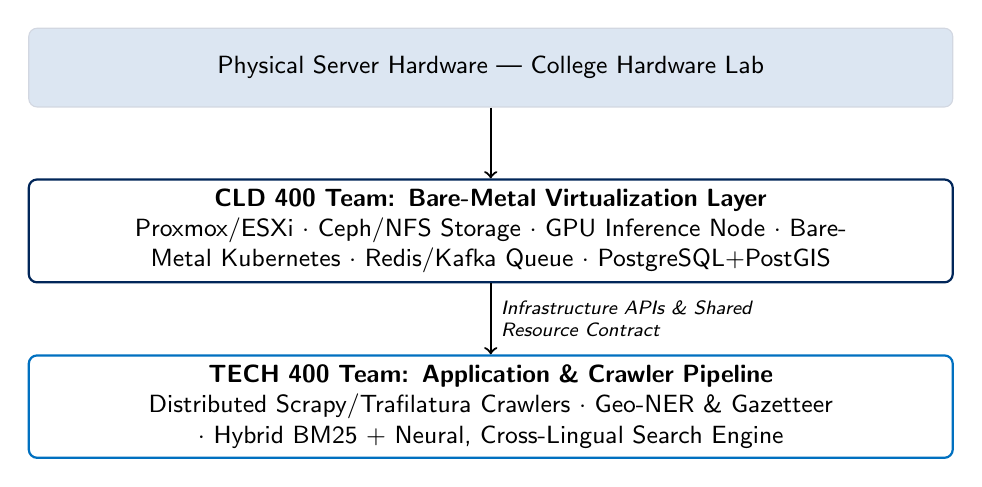
\begin{tikzpicture}[node distance=0.9cm,
  layer/.style={draw=bordergray, fill=lightgray!40, rounded corners=3pt, text width=11.5cm, align=center, minimum height=1cm, font=\small},
  devops/.style={draw=primary, thick, fill=white, rounded corners=3pt, text width=11.5cm, align=center, minimum height=1.3cm, font=\small},
  ir/.style={draw=secondary, thick, fill=white, rounded corners=3pt, text width=11.5cm, align=center, minimum height=1.3cm, font=\small}
]
\node[layer] (hw) {Physical Server Hardware --- College Hardware Lab};
\node[devops, below=of hw] (devops) {\textbf{CLD 400 Team: Bare-Metal Virtualization Layer}\\Proxmox/ESXi $\cdot$ Ceph/NFS Storage $\cdot$ GPU Inference Node $\cdot$ Bare-Metal Kubernetes $\cdot$ Redis/Kafka Queue $\cdot$ PostgreSQL+PostGIS};
\node[ir, below=of devops] (ir) {\textbf{TECH 400 Team: Application \& Crawler Pipeline}\\Distributed Scrapy/Trafilatura Crawlers $\cdot$ Geo-NER \& Gazetteer $\cdot$ Hybrid BM25 + Neural, Cross-Lingual Search Engine};
\draw[->, thick] (hw) -- (devops);
\draw[->, thick] (devops) -- node[right, font=\scriptsize\itshape, text width=3.4cm] {Infrastructure APIs \& Shared Resource Contract} (ir);
\end{tikzpicture}
\end{center}

\subsection*{Shared Resource Contract}
To keep both teams aligned without blocking each other, every cross-layer touchpoint is a strict, named interface:

\begin{table}[H]
\centering
\small
\renewcommand{\arraystretch}{1.25}
\begin{tabularx}{\textwidth}{|>{\bfseries}l|X|X|}
\hline
\rowcolor{lightgray}
Component & Managed By (CLD 400) & Consumed By (TECH 400) \\ \hline
URL Frontier Queue & Redis / Kafka cluster, made highly available & Crawler workers push/pop targeted URLs \\ \hline
Document Storage & Ceph S3-compatible object store / shared NFS & Workers save raw HTML pages \& extracted images \\ \hline
Geo-Database & PostgreSQL + PostGIS instance (master-replica) & System queries/updates geo-tagged news records \\ \hline
Vector \& Text Index & Elasticsearch / Qdrant multi-node cluster & Search backend stores \& queries hybrid indexes \\ \hline
GPU Inference Node & Provisioned, driver/CUDA-installed, and scheduled via the Kubernetes device plugin (Section~\ref{sec:weekly}, Week 1 \& 5) & Serves the dense-embedding and English-to-Nepali translation models as an inference endpoint \\ \hline
Monitoring Dashboard & Grafana (Node Exporter + container stats) & Both teams monitor crawler bandwidth, CPU, and query latency \\ \hline
\end{tabularx}
\end{table}

\subsection*{Four-Phase Joint Execution Strategy}
At a coarser grain than the weekly labs in Section~\ref{sec:weekly}, both teams track four shared milestones:

\begin{table}[H]
\centering
\small
\renewcommand{\arraystretch}{1.3}
\begin{tabularx}{\textwidth}{|X|c|X|X|}
\hline
\rowcolor{lightgray}
Phase & Weeks & CLD 400 Focus & TECH 400 Focus \\ \hline
1: Independent Foundations & 1--4 & Hands-on build-out of the physical stack: hypervisors, networking, distributed storage, Linux HA -- no shared infrastructure exists yet & Full IR theory syllabus (Boolean through language models, classification, and web search) plus from-scratch algorithm prototypes on a small sample corpus -- no live infrastructure to deploy onto yet \\ \hline
2: Joint Integration \& Deployment & 5--6 & Container orchestration, distributed queues/databases, and observability, exposed to the IR team as a shared endpoint & Scale prototypes into real services on the shared cluster: GIS boundary map, full gazetteer, 50+ replica crawler fleet, and real-time geo-tagging \\ \hline
3: Cloud Migration & 7 & Mentor the AWS migration; run a bare-metal-vs-AWS cost/architecture comparison; optionally extend Terraform to target AWS & Learn AWS fundamentals on individually provisioned accounts; migrate and finalize the search engine (heatmaps, bilingual overlay, hybrid ranking) on AWS \\ \hline
4: Full-System Launch \& Defense & 8 & Prove on-premise infrastructure resilience live (kill-node test) during the joint load test & Benchmark search latency (Precision@K, nDCG) and map click-to-render time on the AWS-hosted production system \\ \hline
\end{tabularx}
\end{table}

\subsection*{Information Retrieval System Pipeline}
On top of the shared infrastructure, the TECH 400 build is one continuous pipeline, fanning out into three parallel back ends that converge on a single frontend with two front-door experiences over the same corpus -- click the map, or type a query:

\begin{center}
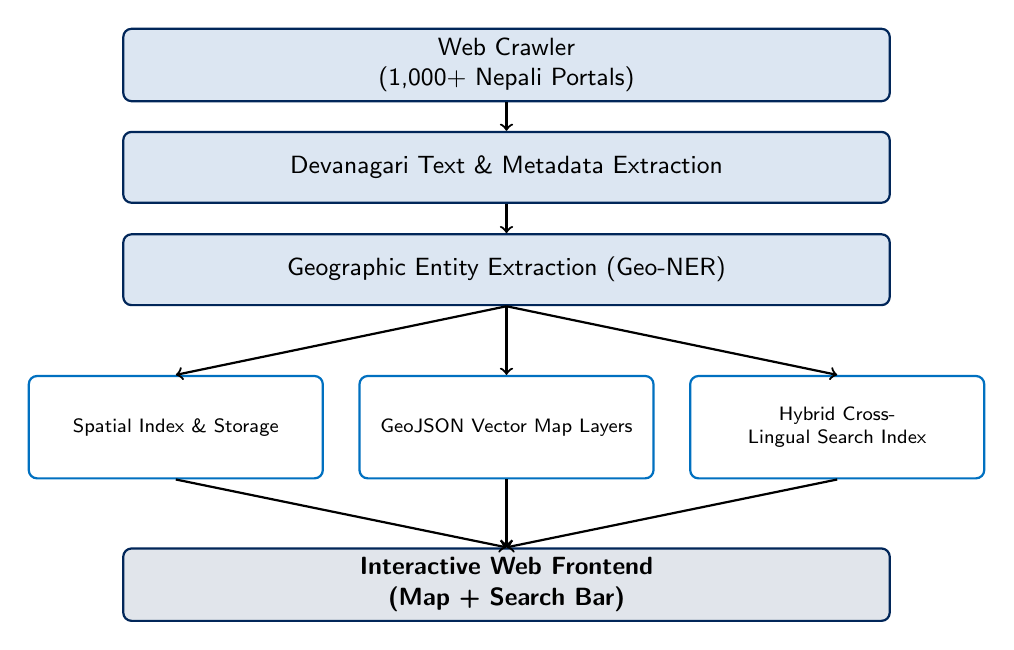
\begin{tikzpicture}[
  stage/.style={draw=primary, thick, fill=lightgray!40, rounded corners=3pt, align=center, text width=9.5cm, minimum height=0.9cm, font=\small},
  branch/.style={draw=secondary, thick, fill=white, rounded corners=3pt, align=center, text width=3.5cm, minimum height=1.3cm, font=\scriptsize},
  final/.style={draw=primary, thick, fill=primary!12, rounded corners=3pt, align=center, text width=9.5cm, minimum height=0.9cm, font=\small\bfseries}
]
\node[stage] (crawler) at (0,8.6) {Web Crawler\\(1,000+ Nepali Portals)};
\node[stage] (extract) at (0,7.3) {Devanagari Text \& Metadata Extraction};
\node[stage] (geoner) at (0,6.0) {Geographic Entity Extraction (Geo-NER)};
\node[branch] (spatial) at (-4.2,4.0) {Spatial Index \& Storage};
\node[branch] (geojson) at (0,4.0) {GeoJSON Vector Map Layers};
\node[branch] (search) at (4.2,4.0) {Hybrid Cross-Lingual Search Index};
\node[final] (frontend) at (0,2.0) {Interactive Web Frontend\\(Map + Search Bar)};
\draw[->, thick] (crawler) -- (extract);
\draw[->, thick] (extract) -- (geoner);
\draw[->, thick] (geoner.south) -- (spatial.north);
\draw[->, thick] (geoner.south) -- (geojson.north);
\draw[->, thick] (geoner.south) -- (search.north);
\draw[->, thick] (spatial.south) -- (frontend.north);
\draw[->, thick] (geojson.south) -- (frontend.north);
\draw[->, thick] (search.south) -- (frontend.north);
\end{tikzpicture}
\end{center}

Five modules make this pipeline real:

\begin{table}[H]
\centering
\small
\renewcommand{\arraystretch}{1.3}
\begin{tabularx}{\textwidth}{|>{\bfseries}l|X|}
\hline
\rowcolor{lightgray}
Module & What Students Build \\ \hline
M1: Hybrid Cross-Lingual Search Engine & Fuse Okapi BM25 with dense neural embeddings (multilingual BERT/LaBSE) into one ranking pipeline behind a search-bar API; detect the query's language and, if it is English, translate it to Nepali with a lightweight HuggingFace MT model before retrieval, so a user typing in either language gets correctly ranked Nepali news back. \\ \hline
M2: Spatial Boundaries \& GIS Layer Processing & Acquire and optimize GeoJSON/TopoJSON boundary data for Nepal's 7 provinces, 77 districts, and 753 municipalities; render interactive boundary polygons (Leaflet.js/MapLibre GL/D3.js) with province $\to$ district $\to$ municipality drill-down navigation. \\ \hline
M3: Geotagging (Spatial NER \& Gazetteer Matching) & Build a structured Devanagari administrative gazetteer covering every province, district, and 753 municipalities, with aliases and colloquial names; implement disambiguation rules resolving partial or alternate place-name mentions to the correct municipality/district/province. \\ \hline
M4: Spatial Indexing \& Storage & Store geo-tagged articles keyed by municipality/district/province ID in PostGIS, or as geo-facets in Elasticsearch/Qdrant; serve a region-filtered REST API such as \texttt{GET /api/v1/news?\allowbreak level=municipality\allowbreak\&id=753\_POKHARA\allowbreak\&sort=latest}. \\ \hline
M5: Heatmaps \& Spatio-Temporal Analytics & News-density heatmaps by region and category filters on the map (e.g., political news in Koshi Province), layered on top of the M1 search bar and M2 map. \\ \hline
\end{tabularx}
\end{table}

% ==========================================
% TEAM ROLES & CROSS-TEAM COMMUNICATION
% ==========================================
\sectionbar{Team Roles \& Cross-Team Communication}
\label{sec:roles}
Both the CLD 400 team and the TECH 400 team are organized like a real engineering organization, not an unstructured group project: a single-person leadership slate per team, plus engineering roles sized to however many students the team actually has.

\subsection*{Leadership Roles (One Student Each)}
Filled from Week 1 (roles may rotate at the midterm checkpoint so every student experiences at least one leadership role):
\begin{itemize}
    \item \textbf{Project Manager} -- Gaurab Thapa (CLD-400) owns the week-by-week timeline, runs stand-ups, and tracks deliverables against this syllabus.
    \item \textbf{Product Owner} -- (Prestige Adhikari (CLD-400)) prioritizes which features matter most for the capstone demo and writes acceptance criteria for each week's deliverable.
    \item \textbf{Solution Architect} -- owns technical design decisions and is the team's point of contact for the Shared Resource Contract (Section~\ref{sec:architecture}) with the other team.
    \item \textbf{Team Lead(s)} -- coordinate day-to-day implementation work and review teammates' code/infrastructure changes.
    \item \textbf{QA} -- owns test plans and benchmark/evaluation suites (MAP/nDCG, failover drills, load tests), and signs off before each week's deliverable is submitted.
\end{itemize}

\subsection*{Engineering Roles (As Many Students as the Team Needs)}
Every deliverable in Section~\ref{sec:weekly} maps onto one of these specialties; a team assigns multiple students to a role when it needs the throughput, and a student may hold an engineering role alongside a leadership one.

\begin{table}[H]
\centering
\small
\renewcommand{\arraystretch}{1.25}
\begin{tabularx}{\textwidth}{|>{\bfseries}l|X|}
\hline
\rowcolor{lightgray}
\multicolumn{2}{|c|}{\textbf{CLD 400 Engineering Roles}} \\ \hline
Network Engineer & VLAN segmentation, LACP bonding, Keepalived/HAProxy, Nginx/Traefik ingress \& MetalLB. \\ \hline
Hardware \& Virtualization Engineer & Proxmox/ESXi provisioning, physical rack \& node setup, the GPU node and its passthrough configuration. \\ \hline
Storage Engineer & Ceph/NFS cluster, RAID policy, PostgreSQL + PostGIS replication and failover. \\ \hline
Kubernetes \& Container Engineer & Docker/Podman images, the K3s/MicroK8s cluster, the NVIDIA GPU device plugin, Helm/manifests. \\ \hline
Observability \& IaC Engineer & Prometheus/Grafana/Loki, and codifying the stack as Terraform/Ansible playbooks. \\ \hline
Cloud Migration Engineer & Week 7--8 AWS mentorship, porting Terraform to AWS, the cost/architecture comparison report. \\ \hline
\end{tabularx}

\vspace{0.6em}

\begin{tabularx}{\textwidth}{|>{\bfseries}l|X|}
\hline
\rowcolor{lightgray}
\multicolumn{2}{|c|}{\textbf{TECH 400 Engineering Roles}} \\ \hline
Crawler \& Data Engineer & Distributed Scrapy/Trafilatura crawlers, Redis/Kafka queue integration, URL dedup at scale. \\ \hline
NLP \& AI Pipeline Engineer & Devanagari NLP, the Geo-NER gazetteer, dense embeddings, and the EN$\to$NE translation model served from the CLD 400 GPU node. \\ \hline
Search \& Ranking Engineer & TF-IDF/BM25/hybrid ranking, MAP/nDCG evaluation, hardening the search endpoint. \\ \hline
Geo-Spatial Engineer & PostGIS/Elasticsearch geo-indexing, spatial queries, GeoJSON/TopoJSON boundary data. \\ \hline
Backend/API Engineer & FastAPI/Node.js REST APIs (\texttt{/api/v1/news}, \texttt{/api/v1/search}). \\ \hline
Frontend/UI Engineer & React/Leaflet/MapLibre map, the search bar, heatmaps, and the bilingual overlay. \\ \hline
\end{tabularx}
\end{table}

\textbf{Cross-team communication (Weeks 1--4):} Even while the two teams work on separate tracks -- CLD 400 building physical infrastructure, TECH 400 covering IR theory and algorithm prototypes -- their Solution Architects and Project Managers hold a short joint stand-up each week to preview the Shared Resource Contract, so the Week 5 integration handoff arrives with no surprises.

% ==========================================
% WEEKLY AT A GLANCE
% ==========================================
\sectionbar{Weekly Schedule at a Glance}
\begin{table}[H]
\centering
\small
\renewcommand{\arraystretch}{1.3}
\begin{tabularx}{\textwidth}{|c|X|X|X|}
\hline
\rowcolor{lightgray}
\textbf{Wk} & \textbf{CLD 400 Theme} & \textbf{TECH 400 Theme} & \textbf{Primary Deliverable} \\ \hline
\multicolumn{4}{|l|}{\textit{Phase 1: Independent Foundations -- separate tracks, weekly cross-team sync}} \\ \hline
1 & Bare-Metal Hypervisors \& Network Foundations & IR Theory I: Boolean Retrieval \& Inverted Indexing & Bonded/VLAN-segmented hypervisor host + Boolean search prototype \\ \hline
2--3 & Enterprise Storage Architecture (Ceph/NFS) & IR Theory II: Vector Space Model, BM25, Evaluation \& Language Models & 3-node Ceph/NFS cluster + TF-IDF/BM25 prototypes benchmarked (MAP/nDCG) \\ \hline
4 & Linux SysAdmin \& High Availability & IR Theory III: Classification, Web Search \& Project Design Review & Keepalived/HAProxy failover + gazetteer/GIS design docs -- Midterm Checkpoint \\ \hline
\multicolumn{4}{|l|}{\textit{Phase 2: Joint Integration \& Deployment -- both teams build on shared infrastructure}} \\ \hline
5 & Containerization \& Bare-Metal Cluster Orchestration & Scale-Up: GIS Boundary Map, Full Gazetteer \& Distributed Crawling & Bare-metal K3s cluster + drill-down map + gazetteer + 50+ replica crawler fleet \\ \hline
6 & Distributed Queues, Database Clustering \& Observability & Real-Time Geo-Tagging \& Hybrid Cross-Lingual Search Engine & Clustered Redis/Kafka + PostGIS/Elasticsearch + Grafana + live geo-tagging + working search bar \\ \hline
\multicolumn{4}{|l|}{\textit{Phase 3--4: Cloud Migration \& Live Defense}} \\ \hline
7 & AWS Mentorship \& Cost/Architecture Comparison & AWS Migration \& Search Engine Hardening & Search engine migrated, hardened \& hosted on individual student AWS accounts \\ \hline
8 & \multicolumn{2}{c|}{Combined Capstone: Production Deployment, Load Testing \& Live Defense} & Full system demo, live on AWS \\ \hline
\end{tabularx}
\end{table}

\newpage

% ==========================================
% WEEKLY COMPREHENSIVE OUTLINE & ASSIGNMENTS
% ==========================================
\sectionbar{Detailed 8-Week Combined Syllabus}
\label{sec:weekly}

\subsection*{Phase 1 Note: Independent Foundations (Weeks 1--4)}
For these four weeks, CLD 400 and TECH 400 run on separate tracks and are graded on separate deliverables: CLD 400 has hands-on physical hardware to build, while TECH 400 has no live infrastructure to deploy onto yet and instead works through the full IR theory syllabus, one algorithm prototype at a time, on a small local sample corpus. Solution Architects and Project Managers from both teams still hold a short weekly stand-up (Section~\ref{sec:roles}) so Week 5's integration handoff has no surprises.

% --- WEEK 1 ---
\subsection*{Week 1: Bare-Metal Hypervisors \& Network Foundations / IR Theory I: Boolean Retrieval \& the Inverted Index}
\textbf{Focus Topics (CLD 400):} Proxmox VE / VMware ESXi bare-metal installation, VLAN segmentation (isolating the crawler network, storage traffic, and public API traffic), LACP network bonding across physical NICs for throughput, and GPU architecture \& virtualization fundamentals (below). \\[0.35em]
\textbf{Focus Topics (TECH 400):} The Boolean retrieval model, inverted index construction, tokenization and Devanagari-aware normalization -- the full theoretical grounding, not yet applied to a live crawler. \\[0.35em]
\textbf{Learning Objective (CLD 400):} Students can partition a bare-metal host into isolated, bonded network segments, and can explain why a GPU node is required to serve the Week 6 translation model. \\[0.35em]
\textbf{Learning Objective (TECH 400):} Students can build a working inverted index by hand -- previewing the gazetteer designed in Week 4 and built in Week 6.

\begin{table}[H]
\centering
\small
\renewcommand{\arraystretch}{1.2}
\begin{tabularx}{\textwidth}{|X|X|}
\hline
\rowcolor{lightgray}
\textbf{CLD 400 Assignment (Virtualization)} & \textbf{TECH 400 Assignment (Information Retrieval)} \\ \hline
\textbf{Lab 1.1: Bare-Metal Hypervisor, Network \& GPU Node Setup} \newline
1. Provision Proxmox VE (or VMware ESXi) on a bare-metal lab server. \newline
2. Configure three VLANs: crawler network, storage traffic (SAN/NAS), and public API traffic. \newline
3. Bond two physical NICs with LACP and benchmark throughput; submit a network topology diagram and benchmark report. \newline
4. Rack and provision a second bare-metal node fitted with a discrete GPU; install NVIDIA drivers and CUDA, and validate GPU passthrough to a test VM/container -- this node will serve the Week 6 translation model. & \textbf{Lab 1.2: Boolean Retrieval Prototype} \newline
1. Assemble a 10--15 document sample corpus of Nepali news text. \newline
2. Implement Devanagari Unicode normalization and a from-scratch Boolean/inverted-index search over the corpus. \newline
3. Submit a short report on where Boolean retrieval breaks down for ambiguous place names, motivating Week 4's design work. \\ \hline
\end{tabularx}
\end{table}

\weeklyreport{Week 1}{Hypervisor/VLAN/LACP theory, your Lab 1.1 build, and your network and GPU-passthrough benchmark results.}{Boolean retrieval/inverted-index theory, your Lab 1.2 implementation, and your corpus/index results.}

\subsection*{GPU Architecture \& Fundamentals (CLD 400 Deep Dive)}
This node is CLD 400's alone to design, build, and defend -- TECH 400 only ever consumes it as an inference endpoint. The deep dive covers:
\begin{itemize}
    \item \textbf{What a GPU is, vs. a CPU:} a handful of powerful, latency-optimized cores (CPU) vs. thousands of simpler, throughput-optimized cores (GPU) built for doing the \emph{same} operation on many data elements at once (SIMT: Single Instruction, Multiple Threads).
    \item \textbf{GPU architecture:} Streaming Multiprocessors (SMs), CUDA cores, warps and thread blocks, the register/shared-memory/global-VRAM hierarchy, and why memory bandwidth -- not just core count -- often bounds real performance.
    \item \textbf{The graphics rendering pipeline:} vertex shading (transforming 3D coordinates), rasterization (converting geometry to pixels), and fragment/pixel shading (coloring/lighting each pixel) -- all independent, parallel, per-vertex or per-pixel work, which is exactly what a GPU is built for.
    \item \textbf{Matrix multiplication as the common core:} 3D rendering is dominated by model-view-projection matrix transforms; neural network layers are dominated by matrix multiply-accumulate (GEMM). Both reduce to the same embarrassingly parallel operation, which is why the same hardware serves both workloads.
    \item \textbf{Why GPUs power AI:} training and inference for models like the Week 6 translation model and dense embedding model are dominated by large matrix multiplications; Tensor Cores add mixed-precision matrix multiply-accumulate units purpose-built for this, orchestrated through CUDA/cuDNN.
    \item \textbf{GPU virtualization:} PCI passthrough (VFIO) to dedicate the physical GPU to one VM; vGPU/MIG (Multi-Instance GPU) to safely share one GPU across tenants; and the Kubernetes NVIDIA device plugin (built in Week 5) that lets pods request a GPU as a schedulable resource.
\end{itemize}

\vspace{0.5em}

% --- WEEK 2-3 ---
\subsection*{Weeks 2--3: Enterprise Storage Architecture (Ceph/NFS) / IR Theory II: Vector Space Model, BM25 \& Evaluation}
\textbf{Focus Topics (CLD 400):} Block vs. object vs. file storage, distributed storage cluster via Ceph or TrueNAS/NFS, RAID 10/6 and Ceph replication policy across physical disks, provisioning persistent volumes for the database and search nodes built in later weeks. \\[0.35em]
\textbf{Focus Topics (TECH 400):} Vector space model and TF-IDF weighting; probabilistic ranking and Okapi BM25; relevance feedback and query expansion; IR evaluation metrics (Precision, Recall, MAP, nDCG); language models for IR. \\[0.35em]
\textbf{Learning Objective (CLD 400):} Students can justify a Ceph/NFS storage design against a RAID-only baseline with measured redundancy data. \\[0.35em]
\textbf{Learning Objective (TECH 400):} Students can prove numerically -- via MAP and nDCG on their own sample corpus -- that BM25 outperforms plain TF-IDF.

\begin{table}[H]
\centering
\small
\renewcommand{\arraystretch}{1.2}
\begin{tabularx}{\textwidth}{|X|X|}
\hline
\rowcolor{lightgray}
\textbf{CLD 400 Assignment (Virtualization)} & \textbf{TECH 400 Assignment (Information Retrieval)} \\ \hline
\textbf{Lab 2.1: Distributed Storage Cluster} \newline
1. Deploy a 3-node Ceph cluster (or TrueNAS/NFS) on lab hardware. \newline
2. Configure RAID 10/6 plus Ceph replication policy across physical disks. \newline
3. Provision a persistent volume and hand off a mount point to the IR team's forthcoming database node; submit a redundancy/failure-injection test report. & \textbf{Lab 2.2: TF-IDF \& BM25 Ranking Prototypes} \newline
1. Implement a from-scratch TF-IDF/cosine-similarity ranking engine over the Week 1 sample corpus. \newline
2. Implement Okapi BM25 over the same corpus and benchmark it against TF-IDF using MAP and nDCG@10. \newline
3. Publish both engines and the benchmark report to GitHub. \\ \hline
\end{tabularx}
\end{table}

\weeklyreport{Weeks 2--3}{Storage-architecture theory (block/object/file, RAID, Ceph replication), your cluster build, and your redundancy/failure-injection results.}{Vector-space/BM25/evaluation theory, your ranking-engine implementation, and your MAP/nDCG benchmark results.}

\newpage

% --- WEEK 4 ---
\subsection*{Week 4: Linux System Administration \& High Availability / IR Theory III: Classification, Web Search \& Project Design Review}
\textbf{Focus Topics (CLD 400):} Kernel tuning for heavy networking (\texttt{sysctl} TCP optimization to sustain thousands of concurrent outgoing crawler sockets), high availability via Keepalived/Virtual IPs and HAProxy load balancing. \\[0.35em]
\textbf{Focus Topics (TECH 400):} Text classification and Na\"ive Bayes; web search fundamentals and PageRank; plus the additional topics this project requires beyond the base IR syllabus -- Geo-NER fundamentals, Devanagari NLP specifics, spatial indexing (PostGIS/quadtrees), and GIS data formats (GeoJSON/TopoJSON) -- covered as design theory ahead of Week 5's build. \\[0.35em]
\textbf{Learning Objective (CLD 400):} Students can keep a service alive through an injected node failure using Keepalived/HAProxy. \\[0.35em]
\textbf{Learning Objective (TECH 400):} Students can produce a gazetteer schema and GIS architecture design ready to be built, not just described, starting Week 5.

\begin{table}[H]
\centering
\small
\renewcommand{\arraystretch}{1.2}
\begin{tabularx}{\textwidth}{|X|X|}
\hline
\rowcolor{lightgray}
\textbf{CLD 400 Assignment (Virtualization)} & \textbf{TECH 400 Assignment (Information Retrieval)} \\ \hline
\textbf{Lab 3.1: Kernel Tuning \& HA Failover} \newline
1. Tune kernel network parameters to sustain 10,000+ concurrent outbound sockets under synthetic crawler load. \newline
2. Deploy Keepalived VIP + HAProxy in front of a sample service. \newline
3. Run and document a live failover drill. & \textbf{Lab 3.2: Classifier Prototype \& Project Design Review} \newline
1. Implement a Na\"ive Bayes classifier over a small labeled sample of news categories. \newline
2. Design (schema-level, not yet built) the Devanagari administrative gazetteer -- every province, district, and 753 municipalities, with aliases -- and its disambiguation rules. \newline
3. Design the GIS boundary-map architecture (GeoJSON/TopoJSON sourcing, drill-down navigation) that Week 5 will implement. \\ \hline
\end{tabularx}
\end{table}

\weeklyreport{Week 4}{Kernel-tuning/HA theory (diagram the Keepalived/HAProxy failover topology), your failover drill, and its results.}{Classification/web-search/Geo-NER theory (with the Na\"ive Bayes math) plus your Lab 3.2 design work; since this week's lab is design-only, the report itself \emph{is} the deliverable.}

\vspace{0.5em}

\subsection*{Midterm Checkpoint (End of Week 4): Architecture \& Integration Review}
Both teams present a system blueprint, not yet an integrated system: the CLD 400 team defends its storage/HA design against the redundancy and failover data collected so far and demonstrates a fully working bare-metal stack (hypervisor, network, storage, HA); the TECH 400 team demonstrates BM25 outperforming TF-IDF on its sample corpus and walks through the Week 4 gazetteer/GIS design docs that Week 5 will build against the now-ready infrastructure.

\newpage

% --- WEEK 5 ---
\subsection*{Week 5: Containerization \& Bare-Metal Cluster Orchestration / Distributed Crawling at Scale}
\textbf{Focus Topics (CLD 400):} Docker and Podman containerization, bare-metal Kubernetes (K3s/MicroK8s), Nginx/Traefik ingress controllers, MetalLB for bare-metal load balancing, and joining the Week 1 GPU node to the cluster via the NVIDIA Kubernetes device plugin. \\[0.35em]
\textbf{Focus Topics (TECH 400):} Web-scale crawling architecture and PageRank; Module 2 (Spatial Boundaries \& GIS Layer Processing) -- acquiring and rendering Nepal's GeoJSON/TopoJSON boundaries with province $\to$ district $\to$ municipality drill-down; Module 3 (Geotagging) -- building the full Devanagari administrative gazetteer at scale from the Week 4 design. \\[0.35em]
\textbf{Learning Objective (CLD 400):} Students can deploy and expose a stateful service on a bare-metal Kubernetes cluster with no public-cloud load balancer. \\[0.35em]
\textbf{Learning Objective (TECH 400):} Students can scale a single-machine crawler into a 50-plus-replica fleet without duplicating work or triggering IP blacklisting, and can render and navigate all three administrative tiers of Nepal on a live web map backed by a complete gazetteer.

\begin{table}[H]
\centering
\small
\renewcommand{\arraystretch}{1.2}
\begin{tabularx}{\textwidth}{|X|X|}
\hline
\rowcolor{lightgray}
\textbf{CLD 400 Assignment (Virtualization)} & \textbf{TECH 400 Assignment (Information Retrieval)} \\ \hline
\textbf{Lab 4.1: Bare-Metal Kubernetes Cluster} \newline
1. Containerize a sample workload with Docker/Podman. \newline
2. Deploy a bare-metal K3s/MicroK8s cluster across the lab's nodes, joining both the standard nodes and the Week 1 GPU node. \newline
3. Install the NVIDIA device plugin so pods can request the GPU as a schedulable resource, and validate with a test inference pod. \newline
4. Configure Nginx/Traefik ingress and MetalLB, and hand off a namespace, a GPU-scheduling-enabled endpoint, and an ingress endpoint to the IR team. & \textbf{Lab 4.2: Distributed Crawler, GIS Map \& Full Gazetteer} \newline
1. Containerize the crawler and deploy it as a 50+ replica Kubernetes Deployment pulling from a single-node Redis queue, with outbound NAT-aware rate limiting and URL deduplication across 1,000+ target portals. \newline
2. Build the interactive Nepal boundary map (province $\to$ district $\to$ municipality drill-down) from real GeoJSON/TopoJSON. \newline
3. Build the complete Nepali administrative gazetteer at scale (every province, district, and 753 municipalities, with aliases) from the Week 4 design, with its disambiguation resolver -- not yet wired into the live pipeline. \\ \hline
\end{tabularx}
\end{table}

\weeklyreport{Week 5}{Kubernetes/GPU-scheduling theory (diagram the cluster topology and GPU device-plugin scheduling path), your cluster build, and your validation results.}{Web-scale crawling/PageRank theory (with the PageRank formula) plus GIS theory, your Lab 4.2 build (code snippets), and its results (map screenshots, gazetteer coverage stats, crawl throughput).}

\vspace{0.5em}

% --- WEEK 6 ---
\subsection*{Week 6: Distributed Queues, Database Clustering \& Observability / Real-Time Geo-Tagging \& Hybrid Cross-Lingual Search}
\textbf{Focus Topics (CLD 400):} Redis/Kafka clustering for high-throughput URL queueing, PostgreSQL + PostGIS with master-replica replication and automated failover, Elasticsearch/Qdrant multi-node shard replication, a full observability stack (Prometheus/Grafana/Loki), and codifying the entire bare-metal stack as Terraform/Ansible playbooks. \\[0.35em]
\textbf{Focus Topics (TECH 400):} Module 3 (Geotagging) -- wiring the Week 5 gazetteer resolver into the live crawl pipeline so every article is geo-tagged in real time; Module 4 (Spatial Indexing \& Storage) -- persisting geo-tagged articles and serving a region-filtered REST API; Module 1 (Hybrid Cross-Lingual Search Engine) -- fusing BM25 with dense neural embeddings and adding automatic English-to-Nepali query translation. \\[0.35em]
\textbf{Learning Objective (CLD 400):} Students can migrate a running crawler fleet onto a clustered, highly available queue and database tier with zero lost URLs. \\[0.35em]
\textbf{Learning Objective (TECH 400):} Students can serve a geographically filtered news query end to end, and can type an English query into the search bar and get back correctly ranked Nepali news via automatic translation.

\begin{table}[H]
\centering
\small
\renewcommand{\arraystretch}{1.2}
\begin{tabularx}{\textwidth}{|X|X|}
\hline
\rowcolor{lightgray}
\textbf{CLD 400 Assignment (Virtualization)} & \textbf{TECH 400 Assignment (Information Retrieval)} \\ \hline
\textbf{Lab 5.1: Clustered Queue, Database \& Observability} \newline
1. Deploy a clustered Redis or Kafka queue with high availability. \newline
2. Deploy PostgreSQL + PostGIS with master-replica replication and automated failover, and a multi-node Elasticsearch/Qdrant cluster with shard replication. \newline
3. Migrate the Week 5 crawler fleet onto the new clustered backend live, with zero downtime. \newline
4. Deploy Prometheus + Grafana + Loki with a live operations dashboard, and codify the entire provisioned stack as Terraform/Ansible playbooks reproducible from bare metal. & \textbf{Lab 5.2: Real-Time Geo-Tagging \& Hybrid Cross-Lingual Search Engine} \newline
1. Wire the gazetteer/Geo-NER resolver into the live crawl pipeline so every ingested article is auto-tagged with province/district/municipality IDs and persisted to PostGIS/Elasticsearch in real time; implement and load-test \texttt{GET /api/v1/news?level=...\&id=...}. \newline
2. Build the hybrid search engine: fuse BM25 with dense neural embeddings (multilingual BERT/LaBSE) into one ranking pipeline behind \texttt{GET /api/v1/search?q=...}. \newline
3. Add automatic query-language detection and English-to-Nepali translation (a lightweight HuggingFace MT model) ahead of retrieval, so the search bar returns correct results regardless of input language. \\ \hline
\end{tabularx}
\end{table}

\weeklyreport{Week 6}{Queueing/HA-database/observability theory (diagram the clustered queue, replication topology, and monitoring stack), your Lab 5.1 build, and its results (failover time, replication lag, dashboard screenshots).}{Geotagging/hybrid-search/cross-lingual-retrieval theory (the BM25-plus-dense-embedding fusion math), your Lab 5.2 build (code snippets), and your search-quality results.}

\newpage

% --- WEEK 7 ---
\subsection*{Week 7: AWS Mentorship \& Cost/Architecture Comparison / AWS Migration, Search Engine Hardening \& Heatmaps}
\textbf{Focus Topics (CLD 400):} AWS fundamentals from a mentor's perspective, mapping bare-metal concepts to their AWS equivalents (EC2 $\approx$ VM, VPC $\approx$ VLAN, S3 $\approx$ Ceph object gateway, RDS $\approx$ managed PostgreSQL+PostGIS); a bare-metal-vs-AWS cost and architecture trade-off analysis; optionally extending the Week 6 Terraform modules to target AWS. \\[0.35em]
\textbf{Focus Topics (TECH 400):} AWS fundamentals (IAM, VPC, EC2, S3, managed/self-hosted search, RDS) on individually provisioned student accounts; Module 5 (Heatmaps \& Spatio-Temporal Analytics); hardening and load-testing the Module 1 search engine ahead of the live defense. \\[0.35em]
\textbf{Learning Objective (CLD 400):} Students can translate their own virtualization expertise into AWS-specific guidance and a defensible cost comparison. \\[0.35em]
\textbf{Learning Objective (TECH 400):} Students can migrate a live production system onto AWS and ship a search bar robust enough to survive unscripted queries during defense.

\begin{table}[H]
\centering
\small
\renewcommand{\arraystretch}{1.2}
\begin{tabularx}{\textwidth}{|X|X|}
\hline
\rowcolor{lightgray}
\textbf{CLD 400 Assignment (Virtualization)} & \textbf{TECH 400 Assignment (Information Retrieval)} \\ \hline
\textbf{Lab 6.1: AWS Mentorship, Cost \& Architecture Comparison} \newline
1. Pair with TECH 400 students as an AWS/infrastructure mentor, mapping each bare-metal component to its AWS equivalent. \newline
2. Produce a bare-metal/Proxmox vs.\ AWS total cost of ownership \& architecture comparison report for a system at this scale. \newline
3. Optionally, extend the Week 6 Terraform modules to provision the equivalent AWS resources, supporting the TECH 400 team's migration. & \textbf{Lab 6.2: Search Engine Hardening, Heatmaps \& AWS Migration} \newline
1. Provision core AWS services (EC2/ECS, S3, a managed or self-hosted search index, RDS or self-hosted PostgreSQL+PostGIS) on your individually assigned AWS account, and migrate the crawler, gazetteer, and search pipeline onto it. \newline
2. Ship the news-density heatmap and category filters on the drill-down map. \newline
3. Load-test and harden \texttt{/api/v1/search}: typo/misspelling tolerance, an empty-result fallback, a defined p95 latency budget, and a graceful fallback from dense to BM25-only search if the embedding service fails. \\ \hline
\end{tabularx}
\end{table}

\weeklyreport{Week 7}{AWS-mentorship/cost-comparison theory (diagram the bare-metal-to-AWS component mapping), your Lab 6.1 work, and your comparison findings.}{AWS-migration/search-hardening theory, your Lab 6.2 work (code snippets), and your load-test/hardening results.}

\vspace{0.5em}

% --- WEEK 8 ---
\subsection*{Week 8: Enterprise Capstone Deployment, Load Testing, \& Defense}
\textbf{Learning Objective (Joint):} Students defend, live, a system they can rebuild from bare metal on command, and can prove -- with numbers, not a slide -- that it works at scale under joint load testing.

\begin{table}[H]
\centering
\small
\renewcommand{\arraystretch}{1.2}
\begin{tabularx}{\textwidth}{|X|}
\hline
\rowcolor{lightgray}
\textbf{Combined Final Capstone Deliverable \& Presentation (CLD 400 + TECH 400)} \\ \hline
\textbf{Production System Defense \& Live Demonstration:} \newline
Both teams deploy their complete, integrated system on the lab hardware and defend it live, together.
\begin{enumerate}
    \item \textbf{Final Presentation (Team Leads only):} On the last day of Week 8, each team's Team Lead presents on behalf of the whole team -- exactly two presenters total, one per team -- covering the architecture, the results, and lessons learned. The resulting score applies equally to every member of that presenter's team. See the rubric in Section~\ref{sec:grading}.
    \item \textbf{Live Crawling Demo (CLD 400 + TECH 400):} Demonstrate continuous ingestion across 1,000+ Nepali portals running on the full clustered queue/storage/Kubernetes stack.
    \item \textbf{Search Accuracy \& Latency (TECH 400):} Report Precision@K and nDCG@10 for the hybrid BM25 + dense-embedding search against the production corpus, including a live, unscripted demo of typing an English query and retrieving correctly ranked Nepali results via automatic translation.
    \item \textbf{GIS Functionality (TECH 400):} Drill down province $\to$ district $\to$ municipality on the live map; a click renders local news with the density heatmap and category filters.
    \item \textbf{Infrastructure Resilience (CLD 400):} Perform a live kill-node test across the on-premise Kubernetes/Ceph/Redis/PostgreSQL stack to prove uninterrupted high availability, independent of the AWS-hosted production deployment.
    \item \textbf{AI-Assisted Engineering Disclosure:} Present the AI Assistance Log required under Section~\ref{sec:ai-policy} and be prepared to explain, unaided, any AI-assisted section of the codebase.
    \item \textbf{Deliverables:} A live, publicly accessible AWS-hosted demo URL, and a production GitHub repository containing Terraform/Ansible code, Kubernetes manifests, the administrative gazetteer, and the full crawler/search pipeline.
\end{enumerate} \\ \hline
\end{tabularx}
\end{table}

\weeklyreport{Week 8}{Full-stack architecture theory (a single diagram of the whole bare-metal system, end to end), your kill-node test, and its results.}{End-to-end evaluation theory, your final benchmark run (code snippets), and its results.} This report is in addition to, not a replacement for, the live defense above.

\vspace{1em}

% ==========================================
% GRADING & ASSESSMENT DISTRIBUTION
% ==========================================
\sectionbar{Combined Assessment \& Grading Scheme}
\label{sec:grading}
Because this course is taught as an integrated dual-subject studio, assessments are split across hands-on system building, infrastructure audits, and technical reporting. Grading is based on demonstrated class performance against this course's own rubrics below -- Westcliff University's standard institutional grading scale and rubrics are not applied to this combined studio for either team. CLD 400 and TECH 400 are graded independently to 100\% each.

\begin{table}[H]
\centering
\small
\renewcommand{\arraystretch}{1.3}
\begin{tabularx}{\textwidth}{|X|c|c|X|}
\hline
\rowcolor{lightgray}
\textbf{Assessment Component} & \textbf{CLD 400 Weight} & \textbf{TECH 400 Weight} & \textbf{Target Learning Outcomes} \\ \hline
Weekly Hands-on Labs \& Reports (Weeks 1--7) & 35\% & 35\% & Practical implementation of distributed storage \& search indexing \\ \hline
Infrastructure Architecture \& IR Technical Reports & 20\% & 20\% & Analysis of virtualization, BM25, storage resilience \\ \hline
Midterm Architecture \& Integration Review (End of Week 4) & 15\% & 15\% & System blueprint \& prototype review \\ \hline
Final Capstone Project \& Live Defense (Week 8) & 30\% & 30\% & Production deployment of the split-team Nepali news engine \\ \hline
\textbf{Total} & \textbf{100\%} & \textbf{100\%} & \textbf{Dual Course Mastery} \\ \hline
\end{tabularx}
\end{table}

\subsection*{Final Capstone Rubric (Week 8): How the 30\% Breaks Down}
\begin{table}[H]
\centering
\small
\renewcommand{\arraystretch}{1.3}
\begin{tabularx}{\textwidth}{|X|c|X|}
\hline
\rowcolor{lightgray}
Sub-Component & Weight & Who Presents / Is Assessed \\ \hline
Final Presentation (Team Leads) & 20\% & Exactly two presenters total -- the CLD 400 Team Lead and the TECH 400 Team Lead, one per team -- each presenting on behalf of their whole team. The score applies equally to every teammate. \\ \hline
Live System Defense \& Technical Q\&A & 10\% & The full team, defending the live crawling demo, search accuracy/latency, GIS functionality, infrastructure resilience, and AI Assistance Log items listed above. \\ \hline
\textbf{Final Capstone Total} & \textbf{30\%} & \\ \hline
\end{tabularx}
\end{table}

\textbf{Final Presentation rubric criteria:} technical depth \& accuracy, live demo quality, communication \& clarity, quality of Q\&A answers (must reflect whole-team understanding, not just the presenter's own work), and professionalism/time management.

\textbf{On "winning":} the instructor may additionally name one team's presentation the strongest of the session -- this is a recognition, not a grading cap. Both teams are scored independently against the rubric above, and \emph{both} can earn the full 20\% (and therefore the full 30\% Final Capstone weight) if both meet the highest criteria; it is not a zero-sum contest.

% ==========================================
% COURSE POLICIES
% ==========================================
\sectionbar{Course Policies \& Engagement Requirements}

\subsection*{Live Session \& Engagement Policy}
Students are required to attend each live 6-hour session in person, as stipulated in Westcliff's institutional course policies.
\begin{itemize}
    \item \textbf{Engagement} is assessed through active participation in the live build session -- pairing, debugging, architecture discussion, and demoing in-progress work -- not through discussion-board word counts, since weekly deliverables in this studio are hands-on labs rather than discussion boards.
    \item \textbf{Missed sessions:} students unable to attend a physical lab session must arrange an in-person make-up session with the instructor before the next class period, since the infrastructure labs depend on shared physical hardware state that cannot be replicated remotely.
\end{itemize}

\subsection*{Assignment \& Reporting Standards}
\label{sec:reporting}
Each lab's deliverable is defined precisely in that week's brief (Section~\ref{sec:weekly}), but every weekly report -- whichever team it comes from -- always has a \textbf{Theory} part and a \textbf{Lab} part, in this shape:
\begin{itemize}
    \item \textbf{CLD 400 reports:} \emph{Theory} -- the concepts behind that week's focus topics, explained with the essential diagrams (network/VLAN topology, storage/RAID layout, cluster architecture, etc.), not prose alone. \emph{Lab} -- your build steps, configuration, and results, wherever a hands-on lab applies that week.
    \item \textbf{TECH 400 reports:} \emph{Theory} -- the complete mathematical and algorithmic grounding for that week's topics (formulas, derivations, pseudocode -- e.g., the BM25 scoring formula, not just its name). \emph{Lab} -- your code snippets, implementation notes, and results (benchmarks, screenshots, evaluation numbers), wherever a hands-on lab applies that week.
    \item Where a week's lab is design-only (e.g., Week 4), the theory and design work together \emph{are} the report -- there is no separate lab-results section to add.
    \item All graded submissions are due by Sunday at 11:59 p.m. Pacific Time, as a PDF or DOC uploaded separately by each team to the course LMS.
    \item The theory section must meet APA 7th-edition formatting (cover page, in-text citations, hanging-indent references) for any external source cited; code and infrastructure artifacts are graded against the rubric published with each lab, not APA formatting.
\end{itemize}

\subsection*{Technical Mentorship \& Writing Center}
\begin{itemize}
    \item The Westcliff University Writing Center supports report and documentation quality, from assignment review to publication help.
    \item Instructor and TA office hours provide code review, architecture feedback, and debugging support for the capstone system throughout all 8 weeks.
\end{itemize}

% ==========================================
% ACADEMIC INTEGRITY & AI POLICY
% ==========================================
\sectionbar{Academic Integrity \& Responsible Generative-AI Use Policy}
\label{sec:ai-policy}
This course assumes students will use AI coding assistants (GitHub Copilot, Claude, GPT-class tools, etc.) as part of a modern engineering workflow, and grades accordingly -- weighting live defense and architectural reasoning far more heavily than static written prose that AI can already produce unaided.

\begin{itemize}
    \item \textbf{Permitted:} Using AI tools for boilerplate scaffolding, syntax lookup, debugging assistance, and drafting documentation.
    \item \textbf{Required disclosure:} Every submission includes a short \textit{AI Assistance Log} noting which components used AI assistance and how.
    \item \textbf{Prohibited:} Submitting AI-generated code, infrastructure, or reports that the student cannot explain, has not tested, or does not understand; presenting AI output as a substitute for the working system itself; sharing or copying a peer's capstone implementation.
    \item \textbf{Live-defense clause:} Any line of submitted code or configuration may be examined orally at any point in the course, including the Week 8 capstone defense. Inability to explain the function, trade-offs, or failure modes of a submitted artifact is treated as an academic integrity concern, regardless of whether AI assistance was disclosed.
    \item \textbf{Standard violations:} Plagiarism of written analysis, fabrication of benchmark or evaluation results, and unauthorized collaboration on individually graded work remain governed by Westcliff University's institutional academic integrity policy.
\end{itemize}

\end{document}
